\documentclass{article}
\usepackage[hyphens]{url}
\usepackage{mathtools}
\usepackage{amsmath}
\usepackage{listings}
\usepackage{graphicx}
\usepackage[margin=1in]{geometry}
\usepackage{float}
\floatstyle{boxed}
\restylefloat{figure}
\lstset{breaklines=true}
\begin{document}


\title{CS595 Intro to Web Science, Assignment \#5}
\author{Valentina Neblitt-Jones}
\date{October 21, 2013}
\maketitle

The ``friendship paradox'' (\url{http://en.wikipedia.org/wiki/Friendship_paradox})  says that your friends have more friends than you do. \\

\section*{Question 1}

Determine if the friendship paradox holds for your Facebook account. Create a graph of the number of friends (y-axis) and the friends sorted by number of friends (x-axis). (The friends don't need to be labeled on the x-axis.) Do include yourself in the graph and label yourself accordingly. \\

Compute the mean, standard deviation, and median of the number of friends that your friends have. \\

You can download your network in an XML file by using the NameGenWeb Facebook app:  \\

\url{https://apps.facebook.com/namegenweb} \\

You will need to give this app permission to access your Facebook data. Make sure you select "Friend Count" as an Extended Attribute. When you download the data, download it in the GraphML format. \\

If you do not have a Facebook account, email me and I will send you my GraphML file.

\subsection*{Answer to Question 1}

My GraphML file is available if necessary, but since it had real names in it I left it on my hard drive instead of loading it to GitHub. When I chose the anonymize option for generating the graph, it also did not provide the friend count so I had to run it without that option. The nodes in the file also contained a unique number for each person and in DoD we would say that it is sufficient for PII violation, but I could find no way to use the number to identify a person in Facebook. I did keep the names on a version of my program because I was curious about who my most popular friend was. Surprise! It was a computer scientist.

I used ElementTree to parse my XML with Python. There was a lot of misunderstanding as I tried to understand how to step through this XML to get at the elements I actually needed.


\begin{figure}[H]
\centering
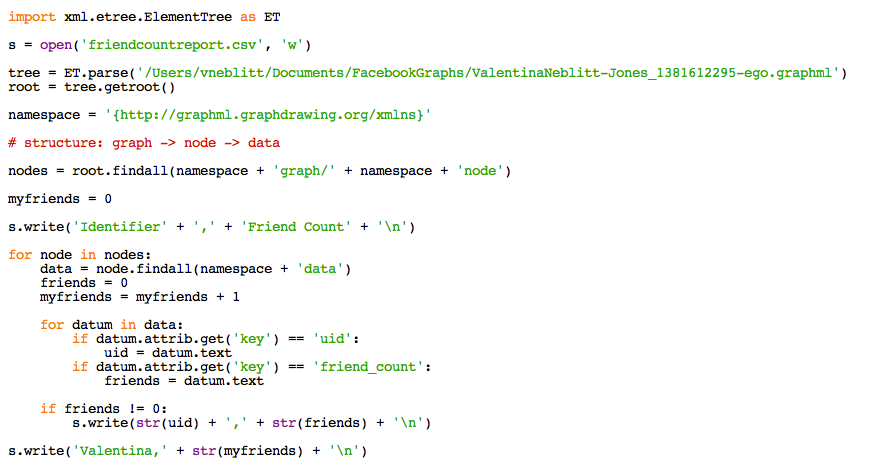
\includegraphics[scale=0.50]{q1/GetFriendCountsCode}
\caption{Showing Friend Count}
\label{GetFriendCountsCode}
\end{figure}

Facebook states that I have 240 friends. The GraphML file only produced 230 friends. I was unable to discover what was at the root of this inaccuracy and what could have been special about the 10 that were left out of the file. \\

However, I was able to figure out a different peculiarity with the data. I discovered when reviewing the GraphML file that some nodes did not contain a Friend Count. I investigated two of those cases and found a difference in summary friends data. Figure \ref{showfriendsprofile} shows a friend whose friend count was in the file and Figure \ref{hidefriendsprofile} shows a friend whose friend count was not in the file. Some of my friends only allow me to see our mutual friends not all of their friends and therefore the application was unable to pull a friend count for those individuals. According to the graph file, I have 230 friends, but my report on friend counts only has 208 of those friends' friend counts. This means that 22 of my friends have the mutual friends only setting. I omitted nodes that did not contain a friend count (Figure \ref{nofriendcount}).

\begin{figure}[H]
\centering

\includegraphics[scale=0.75]{q1/showfriendsprofile}
\caption{Showing Friend Count}
\label{showfriendsprofile}
\end{figure}

\begin{figure}[H]
\centering

\includegraphics[scale=0.75]{q1/hidefriendsprofile}
\caption{Hiding Friend Count}
\label{hidefriendsprofile}
\end{figure}

\begin{figure}[H]
\centering
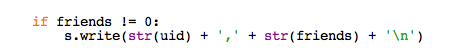
\includegraphics[scale=0.75]{q1/nofriendcount}
\caption{Code that Omits Friends with No Friend Count Available}
\label{nofriendcount}
\end{figure}

I used RStudio to produce the graph for these questions. Figure \ref{friendcountgraph} shows my script to produce the graph. The friends data was sorted via friend count. I needed to set the limit for the y-axis since the default graph tends to not stretch up to the highest number needed. The part about coloring the bar that represented me was tricky. The data was sorted on friend count, but I needed to access identifier which means that I needed to sort on data on a second dimension and keep the first one intact.

\begin{figure}[H]
\centering
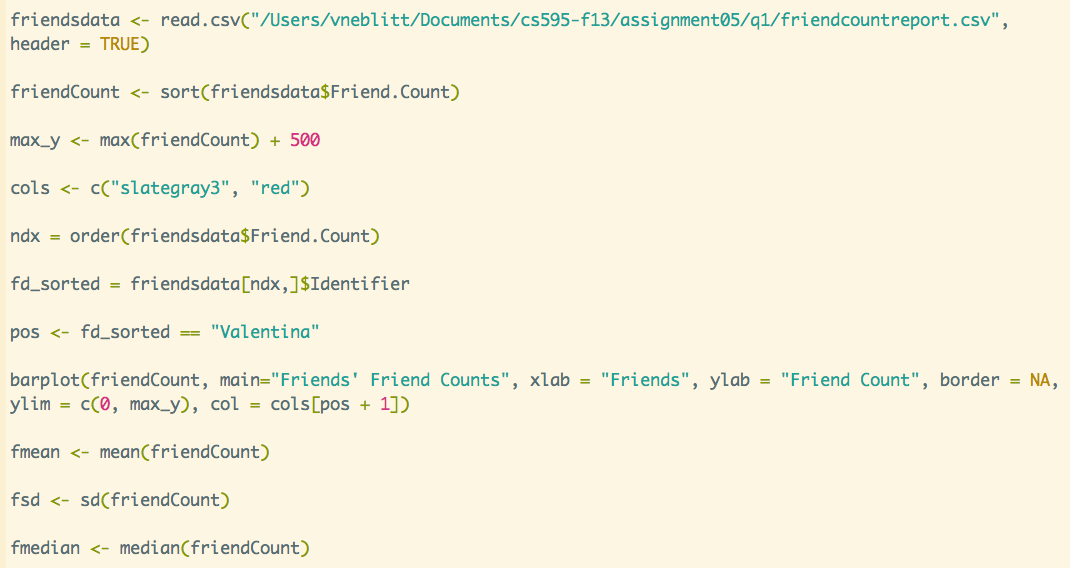
\includegraphics[scale=0.40]{q1/rscriptFB}
\caption{FriendCountGraph.R}
\label{friendcountgraph}
\end{figure}

The graph proved that my friends have more friends than I do. I am represented by the red bar in Figure \ref{friendsfriendcounts}. Figure \ref{statsoutputfriends} shows the part of the R script that calculated the mean, median and standard deviation below.

\begin{itemize}
\item mean = 343.828
\item median = 258
\item standard deviation = 303.303
\end{itemize}

\begin{figure}[H]
\centering
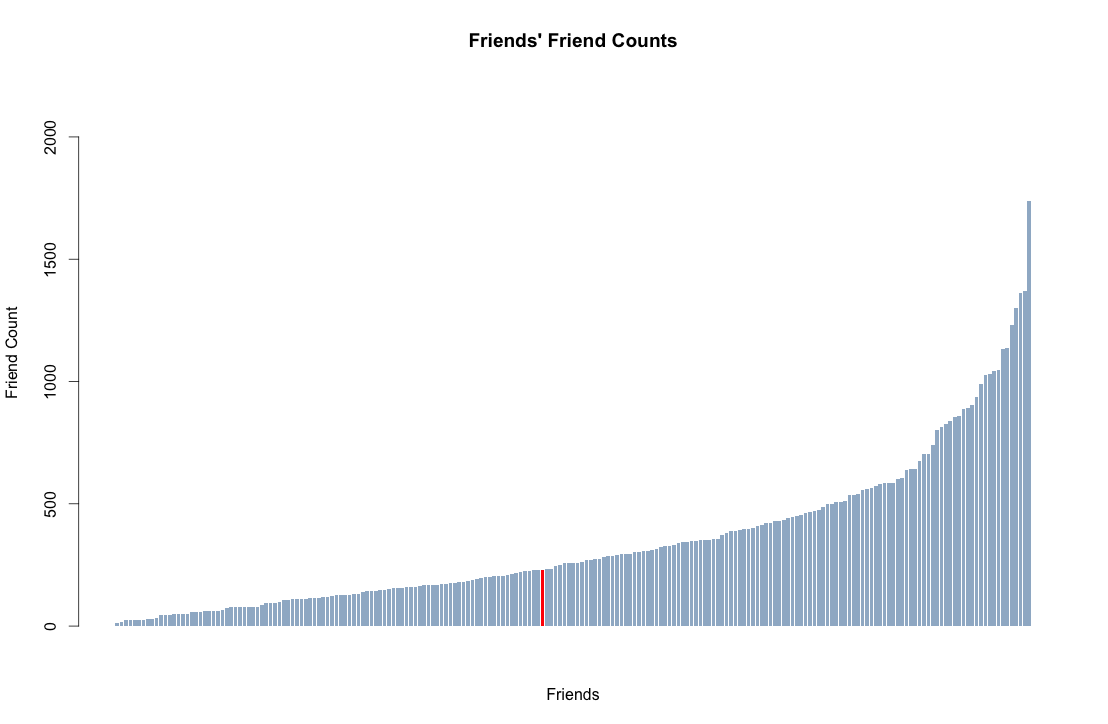
\includegraphics[scale=0.40]{q1/FriendsFriendCounts}
\caption{Facebook Friend Counts}
\label{friendsfriendcounts}
\end{figure}

\begin{figure}[H]
\centering
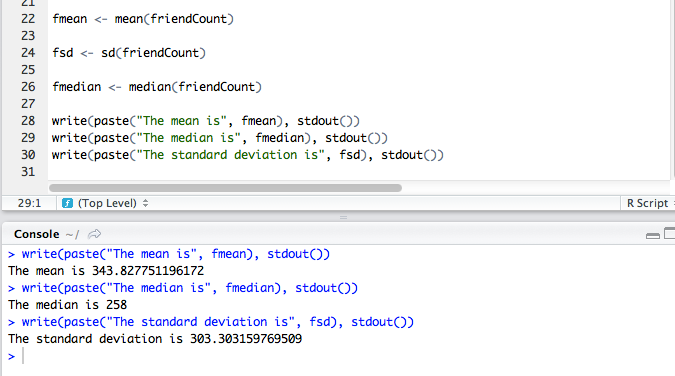
\includegraphics[scale=0.50]{q1/statsoutput}
\caption{Mean, Median, and Standard Deviation}
\label{statsoutputfriends}
\end{figure}


\newpage

\section*{Question 2}

Determine if the friendship paradox holds for your Twitter account. Since Twitter is a directed graph, use ``followers'' as value you measure (i.e., ``do your followers have more followers than you?'') \\

Generate the same graph as in question \#1, and calculate the same mean, standard deviation, and median values. \\

For the Twitter 1.1 API to help gather this data, see: \\

\url{https://dev.twitter.com/docs/api/1.1/get/followers/list} \\

If you do not have followers on Twitter (or don't have more than 20), then use my Twitter account ``phonedude\_mln''.

%\begin{table}[!h]
%\centering
%\caption{10 Hits for the term ``shadow'', ranked by TFIDF}
%\begin{tabular}{c c c c}
%\hline
%TFIDF & TF & IDF & URI \\
%\hline
%\hline
%0.150 & 0.014 & 10.680 & http://foo.com \\
%0.085 & 0.008 & 10.680 & http://bar.com \\
%\hline
%\end{tabular}
%\end{table}

\subsection*{Answer to Question 2}

My own Twitter account did not come close to meeting the threshold for this assignment. I am following 23 and only have 6 followers. So I used phonedude\_mln. The top part of the code is identical to the work for Assignment \#2 Question \#1. Therefore Figure \ref{GetFollowersCode} shows the part that is different. The JSON format (Figure \ref{jsonformat}) showed that I needed to get the ``followers\_count'' to gather the data for this question.

\begin{figure}[H]
\centering
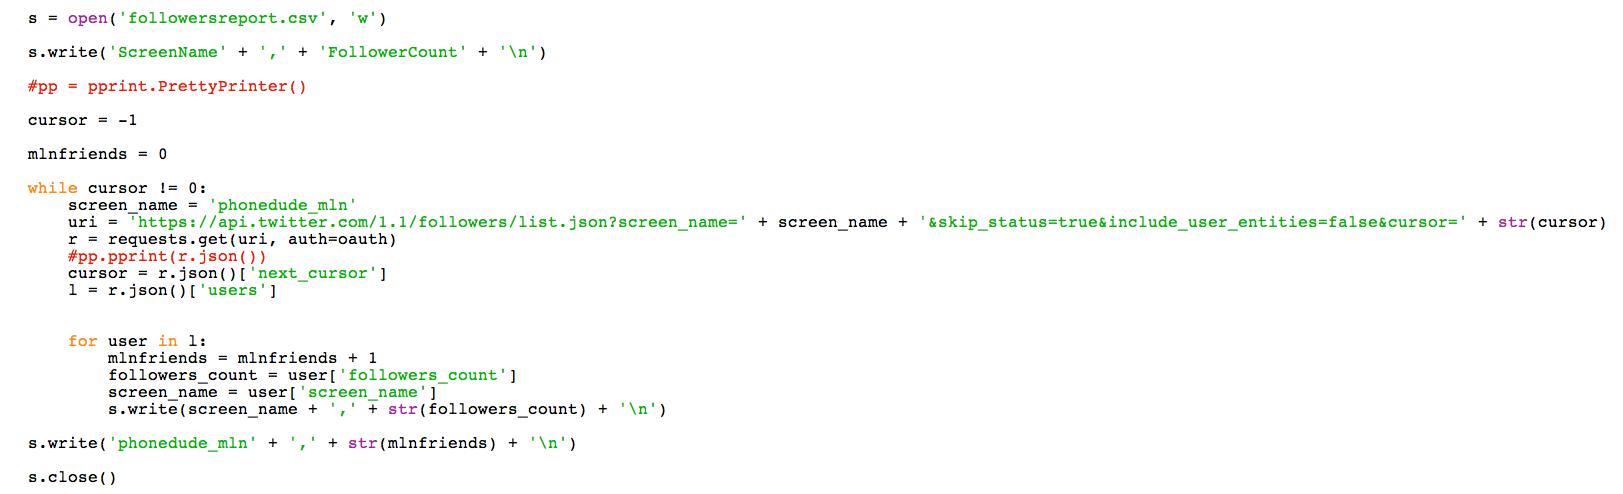
\includegraphics[scale=0.25]{q2/GetFollowersCode}
\caption{GetFollowers.py}
\label{GetFollowersCode}
\end{figure}

\begin{figure}[H]
\centering
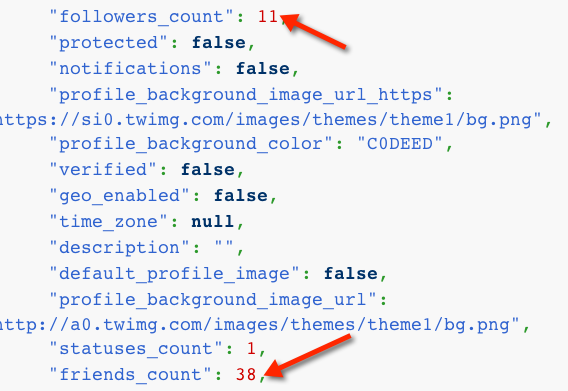
\includegraphics[scale=0.50]{q2/jsonformat}
\caption{JSON Format}
\label{jsonformat}
\end{figure}

I was able to mostly reuse the code from Question \#1 for this graph. I had to change input file, graph labels and variable names. Again the red bar on Figure \ref{followercounts} represents phonedude\_mln.

\begin{itemize}
\item mean = 515.197
\item median = 196
\item standard deviation = 1251.050
\end{itemize}

\begin{figure}[H]
\centering
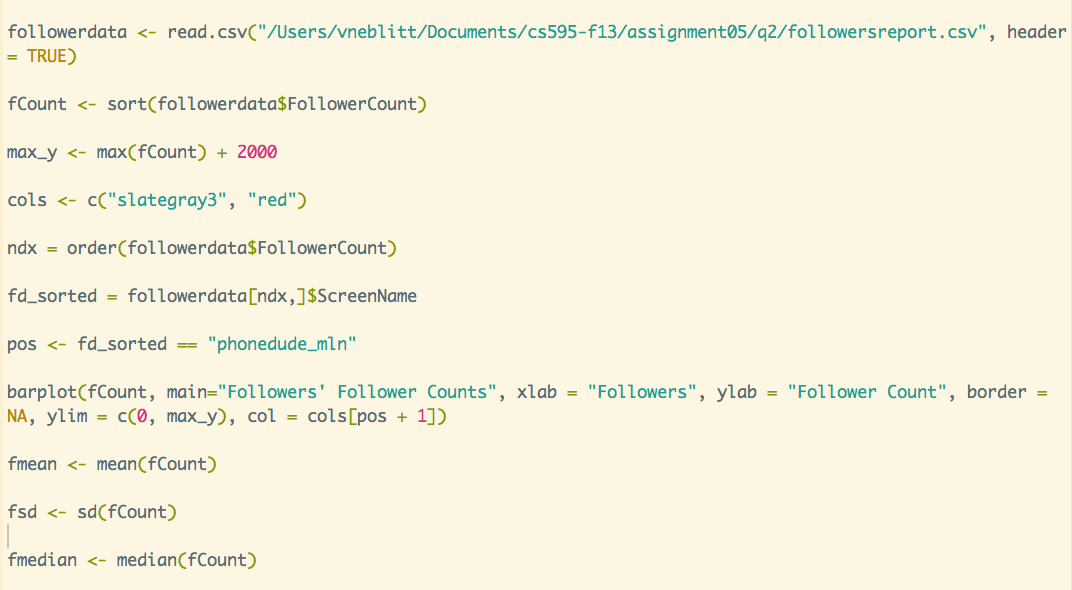
\includegraphics[scale=0.40]{q2/rscriptTfollowers}
\caption{FollowerCountGraph.R}
\label{followercountgraph}
\end{figure}

\begin{figure}[H]
\centering
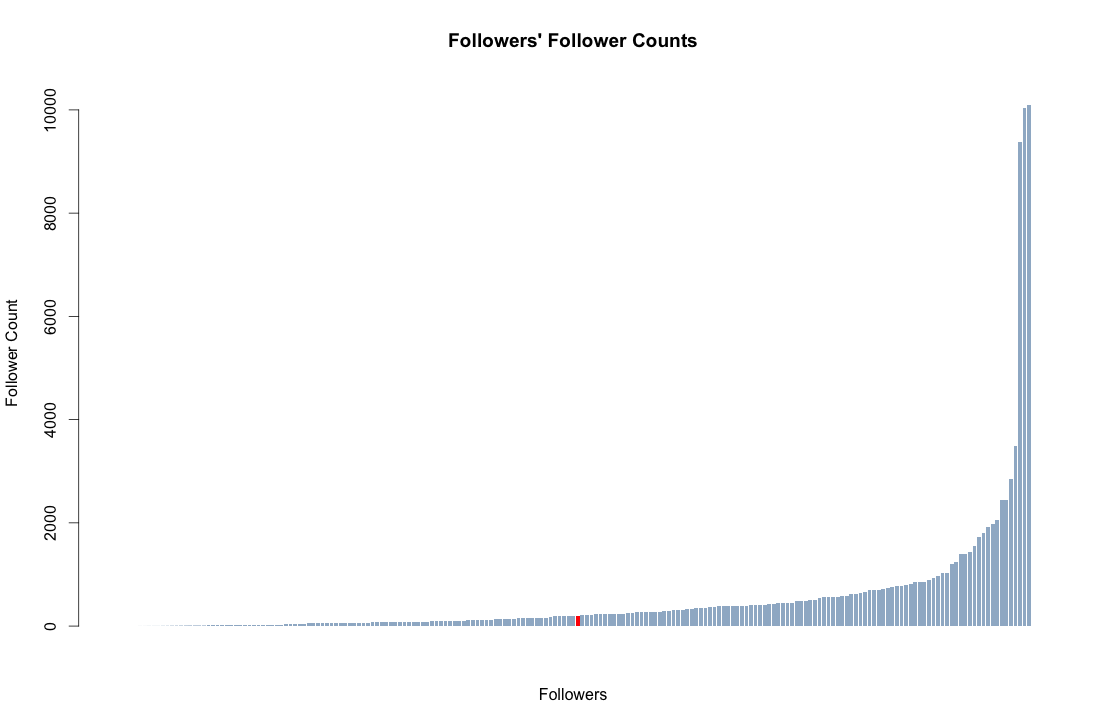
\includegraphics[scale=0.38]{q2/FollowerCountGraph}
\caption{Twitter Followers Count}
\label{followercounts}
\end{figure}

\begin{figure}[H]
\centering
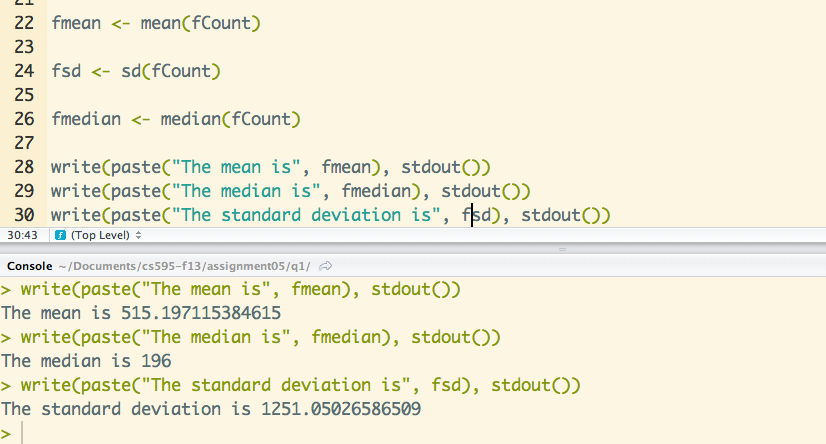
\includegraphics[scale=0.50]{q2/statsoutput}
\caption{Mean, Median, and Standard Deviation}
\label{statsoutputfollowers}
\end{figure}

\clearpage

\section*{Extra Credit - LinkedIn (2 points)}

Repeat question \#1, but with your LinkedIn profile.

\subsection*{Answer to Extra Credit - LinkedIn}

Not attempted.

\clearpage

\section*{Extra Credit - Twitter (1 point)}

Repeat question \#2, but change ``followers'' to ``following''? In other words, are the people I am following following more people?

\subsection*{Answer to Extra Credit - Twitter}

Again I had to use phonedude\_mln and the top part of the code is identical to the work for Assignment \#2 Question \#1. Therefore Figure \ref{GetFollowingCode} shows the part that is different. This time I needed the ``friends\_count'' data from the output (Figure \ref{jsonformat}).

\begin{figure}[H]
\centering
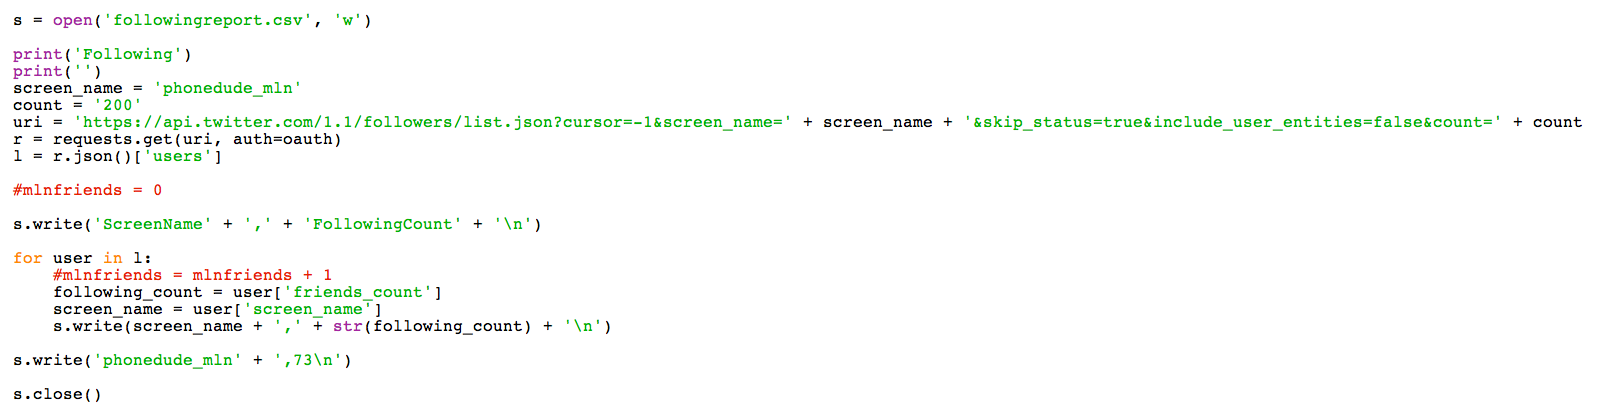
\includegraphics[scale=0.25]{e2/GetFollowingCode}
\caption{GetFollowing.py}
\label{GetFollowingCode}
\end{figure}

Again, I was able to mostly reuse the code from Question \#1 for this graph. I had to change input file, graph labels and variable names. The red bar on Figure \ref{followingcounts} represents phonedude\_mln.

\begin{itemize}
\item mean = 512.627
\item median = 287
\item standard deviation = 578.277
\end{itemize}

\begin{figure}[H]
\centering
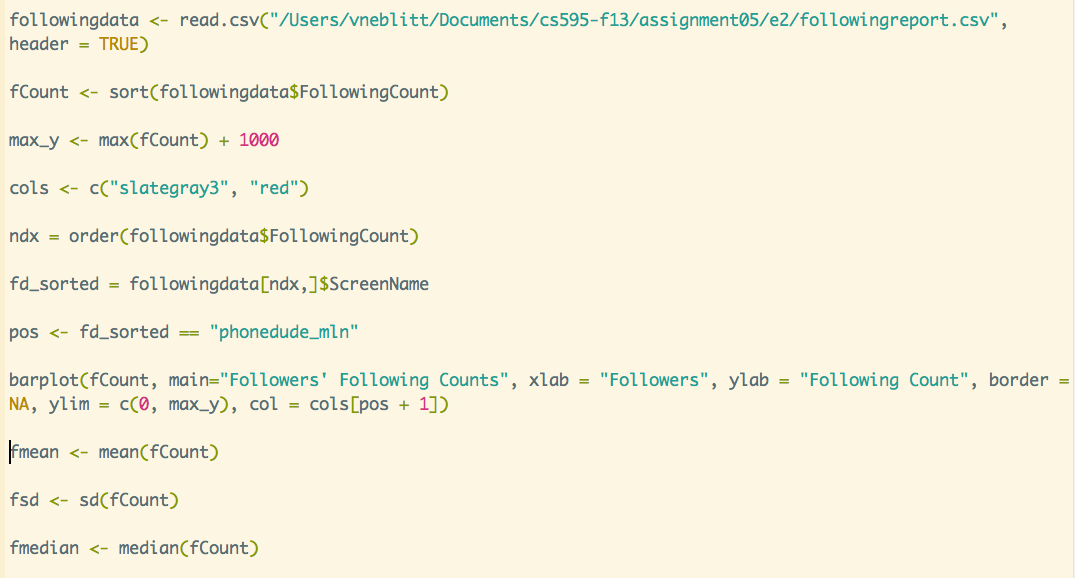
\includegraphics[scale=0.40]{e2/rscriptTfollowing}
\caption{FollowingCountGraph.R}
\label{followingcountgraph}
\end{figure}

\begin{figure}[H]
\centering
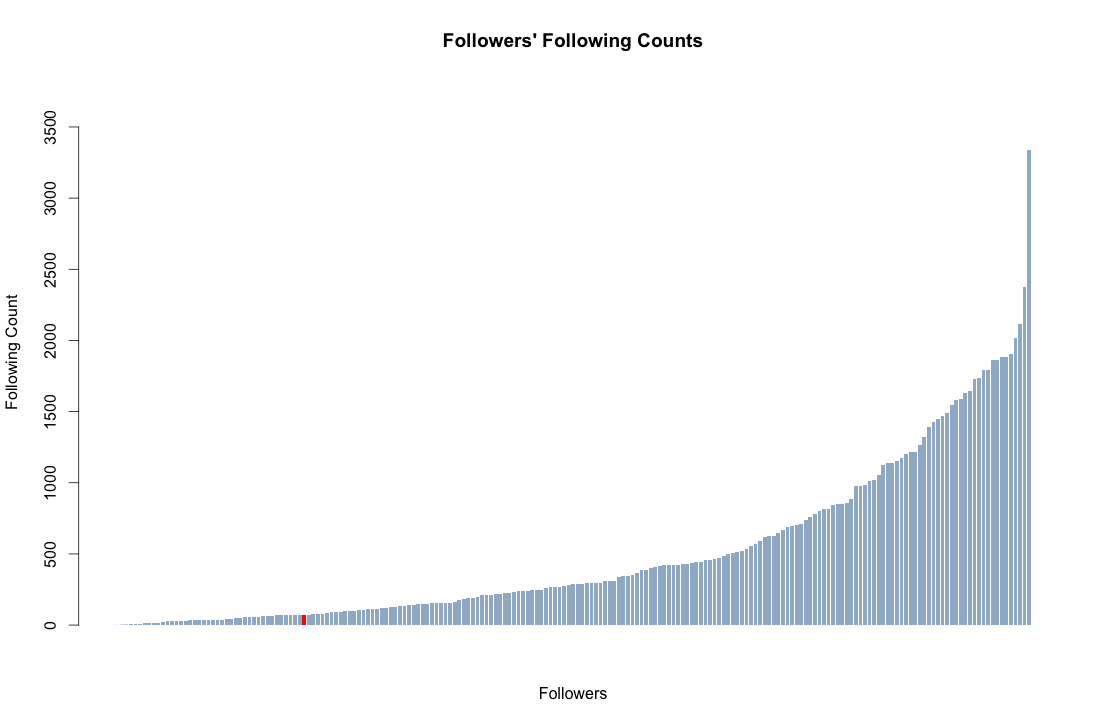
\includegraphics[scale=0.40]{e2/FollowingCountGraph}
\caption{Twitter Following Count}
\label{followingcounts}
\end{figure}

\begin{figure}[H]
\centering
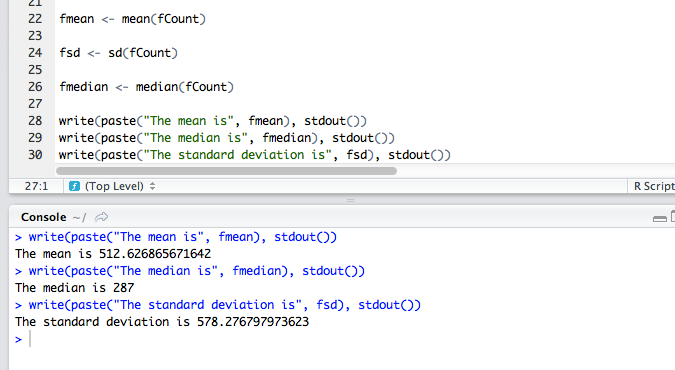
\includegraphics[scale=0.50]{e2/statsoutput}
\caption{Mean, Median, and Standard Deviation}
\label{statsoutputfollowing}
\end{figure}


\clearpage

\section*{Resources}

\begin{itemize}
\item Grosfield, Troy. Parsing XML with Python using ElementTree. \url{http://blog.troygrosfield.com/2010/12/18/parsing-xml-with-python-using-elementtree/}
\item McCown, Frank. Producing Simple Graphs with R. \url{http://www.harding.edu/fmccown/r/}
\item Poulson, Barton. R Statistics Essential Training. \url{http://www.lynda.com/course20/R-tutorials/R-Statistics-Essential-Training/142447-2.html}
\item Python.org. The ElementTree XML API. \url{http://docs.python.org/3.3/library/xml.etree.elementtree.html}
\item Seminar for Statistics. R Documentation: Arithmetic Mean. \url{http://stat.ethz.ch/R-manual/R-devel/library/base/html/mean.html}
\item Seminar for Statistics. R Documentation: Concatenate Strings. \url{http://stat.ethz.ch/R-manual/R-devel/library/base/html/paste.html}
\item Seminar for Statistics. R Documentation: Median Value. \url{http://stat.ethz.ch/R-manual/R-patched/library/stats/html/median.html}
\item Seminar for Statistics. R Documentation: Standard Deviation. \url{http://stat.ethz.ch/R-manual/R-patched/library/stats/html/sd.html}
\item Stack Overflow. Change colors or particular bars in a bar chart. \url{http://stackoverflow.com/questions/13112974/change-colours-of-particular-bars-in-a-bar-chart}
\item Stack Overflow. How do you print to stderr in R? \url{http://stackoverflow.com/questions/1109017/how-do-you-print-to-stderr-in-r}
\item Stack Overflow. Understanding the Order() function in R. \url{http://stackoverflow.com/questions/2315601/understanding-the-order-function-in-r}
\item Twitter Developers Documentation. GET followers/list. \url{https://dev.twitter.com/docs/api/1.1/get/followers/list}
\item Twitter Developers Documentation. Using cursors to navigate collections. \url{https://dev.twitter.com/docs/misc/cursoring}
\end{itemize}

\end{document}